%% Empirical Economics submission (Springer Nature sn-jnl template)
\documentclass[pdflatex,sn-basic]{sn-jnl}

\usepackage{amsmath,amssymb}
\usepackage{booktabs}
\usepackage{graphicx}
\usepackage{url}
\let\orcidlogo\relax
\usepackage{orcidlink}
\graphicspath{{figures/}}

%% Anonymous version: create an empty file blind.flag before compiling
\newif\ifblind
\blindfalse
\IfFileExists{blind.flag}{\blindtrue}{}

\raggedbottom

\begin{document}

\title[Country panels and broadband price responsiveness]{What can country panels tell us about broadband price responsiveness? Evidence from the European Union and the Eastern Partnership, 2010--2024}

\ifblind
\author{Anonymous}
\affil{Anonymous}
\else
\author*[1,2,3]{\fnm{Samir} \sur{Orujov}\,\orcidlink{0009-0004-9708-2109}}\email{sorujov@ada.edu.az}
\author[2,4]{\fnm{Ilgar} \sur{Ismayilov}}
\author[2]{\fnm{Jeyhun} \sur{Huseynzade}}
\affil*[1]{\orgdiv{School of Business}, \orgname{ADA University}, \orgaddress{\city{Baku}, \country{Azerbaijan}}}
\affil[2]{\orgname{Information Communication Technologies Agency}, \orgaddress{\city{Baku}, \country{Azerbaijan}}}
\affil[3]{\orgname{CERGE-EI, a joint workplace of Charles University and the Economics Institute of the Czech Academy of Sciences}, \orgaddress{\city{Prague}, \country{Czech Republic}}}
\affil[4]{\orgdiv{Faculty of Social Sciences}, \orgname{Charles University}, \orgaddress{\city{Prague}, \country{Czech Republic}}}
\fi

\abstract{Regulators often judge how strongly broadband adoption responds to price from country panels, because comparable household data are scarce. We examine what such a panel can reveal, using ITU entry-level price baskets for 27 European Union (EU) and six Eastern Partnership (EaP) countries over 2010--2024. A two-way fixed-effects regression of log subscriptions on log prices gives a sizeable negative coefficient whose year-specific values rise steadily towards zero and above, a pattern that suggests broadband has become a necessity. A simulation with no price effect reproduces this pattern when late adopters start with high prices, and the pattern disappears in the data once country-specific trends are removed or the model is estimated in differences. In the EU the association between entry-level prices and adoption is then close to zero throughout; the 90\% confidence interval in first differences is $[-0.04, 0.02]$. In the EaP adoption grew fastest in the years in which affordability improved most, giving coefficients between $-0.17$ and $-0.46$. This association rests on movements common to the six countries: with EaP-specific year effects it vanishes, and with small-sample inference it is fragile. Regional data for 175 EU regions show no stronger association in less-developed regions. Country panels of this kind do not identify a price response, and they give no evidence of a break in 2020.}

\keywords{Broadband adoption, Affordability, Technology diffusion, Panel data, Small-sample inference, Eastern Partnership}

\pacs[JEL Classification]{L96, C23, O33, L51}

\maketitle

\section{Introduction}\label{sec:intro}

Whether the adoption of fixed broadband still responds to its price matters for telecommunications regulation. If it does, affordability instruments such as social tariffs, subsidies and the universal-service provisions of the European Electronic Communications Code \citep{eecc2018} are effective ways of widening access. If it does not, the binding constraints lie elsewhere, in availability, quality or skills. The Broadband Commission target that entry-level broadband should cost less than 2\% of monthly gross national income (GNI) per capita \citep{broadbandcommission2018} presumes that price matters.

The most credible estimates come from household data, usually stated-preference surveys or discrete-choice models for a single country \citep{rosston2010household,cardona2009demand,ida2008discrete,grzybowski2014market,liu2018distinguishing}. Such data are rarely comparable across countries. Regulators and international organisations therefore often use country panels built from the International Telecommunication Union (ITU) price baskets and subscription counts, which are public, harmonised and complete. In such panels, however, prices and adoption move together for many reasons besides demand, and the variation within a country is dominated by its own slow path of diffusion \citep{griliches1957hybrid,geroski2000models,comin2010exploration}.

This article asks what a country panel of this kind can reveal about the price responsiveness of adoption. We study the 27 member states of the European Union and the six countries of the Eastern Partnership (Armenia, Azerbaijan, Belarus, Georgia, Moldova and Ukraine) between 2010 and 2024. The two groups began the period at different points of the diffusion curve. In 2010--2013, EaP penetration averaged 12 subscriptions per 100 inhabitants and entry-level broadband cost 4.1\% of monthly GNI per capita; the corresponding EU figures were 26 and 1.2\%.

We report four findings. First, the two-way fixed-effects (TWFE) regression of log subscriptions on log prices gives a pooled coefficient of $-0.23$ for 2010--2019, and its year-specific version rises monotonically from $-0.43$ in 2010 to $+0.15$ in 2024. This is easily read as evidence that broadband became a necessity. A simulation in which price has no effect at all, but late adopters start with high prices, produces the same kind of pattern, and in the data the pattern disappears once country-specific trends are allowed or the model is estimated in differences. Second, in the EU the coefficient on entry-level prices is close to zero in every such specification, in long differences and in country-by-country estimates. A regional panel of 175 EU regions shows no stronger association in less-developed regions, although it cannot rule out a moderate one. Third, in the EaP the coefficient remains negative in most specifications, between $-0.17$ and $-0.46$. It reflects the fact that EaP adoption grew fastest in the years in which EaP affordability improved most, in particular 2011--2013. When year effects are allowed to differ between the EaP and the EU, so that the EaP coefficient is identified only from differences among the six EaP countries, it is $+0.13$ and insignificant. With six countries, inference is delicate, and the permutation and wild-bootstrap $p$-values for the EaP--EU difference range from 0.005 to 0.52 across specifications. Fourth, there is no evidence of a break in 2020.

We draw two conclusions. For the question that regulators ask, a country panel of this kind is not informative: it identifies a price response neither in mature markets nor in markets that are catching up, and apparent changes in the response over time are easily produced by diffusion. For empirical practice, levels regressions of this kind should be reported together with trend-robust and differenced estimates, and inference on small groups of countries should use methods designed for few clusters. The article thus contributes a documented example, with public data, of how a standard design misleads, together with the diagnostics that reveal it.

Section~\ref{sec:background} reviews the evidence and the policy setting. Section~\ref{sec:data} describes the data, including two features of the ITU price series that matter for estimation. Section~\ref{sec:method} sets out the estimators and the inference, Section~\ref{sec:results} presents the results, Section~\ref{sec:discussion} discusses them, and Section~\ref{sec:conclusion} concludes.

\section{Background}\label{sec:background}

\subsection{Evidence on broadband demand}

Table~\ref{tab:lit} summarises estimates that bear on the price sensitivity of broadband demand. Household studies find large own-price elasticities for particular technologies. \citet{cardona2009demand} report elasticities for DSL between $-0.97$ and $-2.55$ in Austria, depending on the presence of cable competition, and \citet{grzybowski2014market} obtain about $-3.0$ for DSL and $-2.0$ for fixed broadband as a whole in Slovakia. These elasticities concern the choice between technologies and providers, which is more sensitive to price than the decision to be connected at all. Studies of willingness to pay \citep{rosston2010household,liu2018distinguishing,sinclair2023assessing} show that valuations of speed and reliability are high, concave in speed and rising over time; \citet{lindlacher2021low} finds that many German households do not upgrade to faster plans where these are available. Evidence on subsidies is closer to the margin studied here: \citet{mendez2021lifeline} estimate that the US Lifeline subsidy of US\$9.25 per month raised adoption among low-income households by about 6\%, a modest effect for a sizeable price reduction. On the supply side, \citet{wilson2025public} shows that municipal entry crowds out private fibre investment.

Cross-country evidence is scarcer. \citet{galperin2013price} use a cross-section of Latin American and Caribbean countries with instrumental variables and find that adoption is price-elastic there but not in the OECD comparison group. \citet{dauvin2014estimating} study diffusion across EU regions in 2006--2010 and relate its speed to competition and access regulation rather than to a single elasticity, and \citet{lyons2014timing} examines the timing and local determinants of residential broadband adoption in Ireland. The present article belongs to this cross-country strand, but its question is what a country panel can identify at all. The answer draws on the view of adoption as a diffusion process \citep{griliches1957hybrid,geroski2000models,comin2010exploration}, in which prices, incomes and adoption trend together within countries, and on the recent literature showing that TWFE estimators average heterogeneous effects with weights that need not be intuitive, including when the regressor is continuous \citep{dechaisemartin2020two,goodman2021difference,callaway2024difference}.

\subsection{Affordability policy in the EU, the United States and the Eastern Partnership}

In the EU, regulation has concentrated on the supply side: access regulation, the reduction of deployment costs \citep{bcrd2014}, now under the Gigabit Infrastructure Act \citep{gia2024}, and state aid for rural networks. Affordability enters mainly through Article~84 of the European Electronic Communications Code, which requires member states to ensure that adequate broadband is affordable for consumers on low incomes \citep{eecc2018}. The instruments are targeted social tariffs and direct support; retail broadband prices are otherwise largely unregulated. Empirical work on European broadband policy has correspondingly focused on access regulation and investment \citep{briglauer2018speeding,wallsten2006broadband}.

The United States has relied more on demand-side subsidies. Lifeline has supported telephone and later broadband service for low-income households for decades, and the Affordable Connectivity Program, created by the Infrastructure Investment and Jobs Act of 2021, subsidised the bills of more than twenty million households until its funding was exhausted in 2024 \citep{fcc_acp}. The evaluation literature on such programmes is thin \citep{hauge2010demand}, and the estimated adoption effects are modest \citep{mendez2021lifeline}.

The six EaP countries differ from the EU in two respects. At the start of the period incomes were a fraction of EU incomes, so the affordability ratio was far higher. In several of them the incumbent fixed-line operator was, and in some cases still is, state-owned, so entry-level tariffs were partly administered rather than set in competitive markets. Regulatory convergence with the EU has been pursued through the EU4Digital initiative and the network of EaP regulators, EaPeReg \citep{eu4digital}, with an emphasis on market analysis, spectrum and roaming rather than retail price control; Belarus suspended its participation in the Eastern Partnership in 2021. For these regulators, whether entry-level prices still govern adoption decides whether affordability should remain a priority.

\section{Data}\label{sec:data}

\subsection{Adoption and prices}

The sample consists of the 27 EU member states and the six EaP countries in 2010--2024, 495 country-years. Adoption is measured by fixed-broadband subscriptions per 100 inhabitants, the ITU indicator as distributed by the World Bank in its July 2026 release \citep{worldbank2026wdi}. The value for Bulgaria in 2024 is missing and is left missing.

Prices are the ITU fixed-broadband baskets \citep{itu2025baskets,itu2020measuring}. The basket is the monthly price of the cheapest plan offered by the operator with the largest market share that provides at least a minimum monthly data allowance at an advertised speed of at least 256\,kbit/s. It excludes installation and equipment charges; a bundle is used if it is the cheapest way to meet the threshold. ITU reports the price in US dollars at market exchange rates, in purchasing-power-parity (PPP) dollars, and as a percentage of monthly GNI per capita. The last is the affordability measure of the Broadband Commission target and is our main price variable.

Two features of the series matter. First, the minimum allowance was raised from 1\,GB to 5\,GB in 2018, and ITU warns that values from 2018 onwards are not directly comparable with earlier ones \citep{itu2020measuring}. We therefore never use the change from 2017 to 2018 in differenced regressions, and we report estimates separately for the two definitions. Second, for 22 of the 33 countries the ITU workbook reports in 2019 exactly the 2018 values in all three units; we treat these repeated values as missing. The Romanian value for 2013 is missing in the source. No price or subscription value is imputed.

The basket is an entry-level price. Beyond the thresholds it does not hold quality fixed, and as subscribers move to faster plans it becomes less representative of what they pay. It is best viewed as the cost of basic access, which is the margin relevant to adoption and to affordability policy.

\subsection{Controls}

The core controls capture shifts in demand and in the cost of supply that could move prices and adoption together. On the demand side, log GDP per capita in current US dollars measures income; the urban share of the population and the gross tertiary enrolment rate measure the concentration of demand and digital skills; the share of the population aged 15--64 measures household composition; GDP growth and inflation (GDP deflator) capture cyclical conditions and the real value of nominal tariffs. On the supply side, log population density measures the cost of deployment, and the World Bank regulatory-quality index \citep{worldbank2026wdi} measures the institutional environment for entry and investment. Secure internet servers per million inhabitants and research and development expenditure, used in earlier work on this panel, are plausibly consequences of broadband diffusion; we exclude them from the main specification and add them in a robustness check. Tertiary enrolment has 30 missing values (6\% of the panel), filled by linear interpolation within countries or, at the ends of a country's series, by the nearest observed value. No other core control has gaps.

Official income statistics for some EaP economies are subject to large revisions and exchange-rate swings. As a control that does not depend on national accounts we use night-time lights \citep{henderson2012measuring}, whose relation to GDP differs across countries \citep{phan2023lights}, taken from the harmonised DMSP/VIIRS series of \citet{li2020harmonized} in its 2024 release, summed over each national territory and divided by population. Because the series switches from DMSP to simulated VIIRS data in 2014, the 2013--2014 change is excluded whenever lights enter in differences. Annual changes in lights and in GDP per capita have a correlation of 0.25.

\subsection{Regional data}

For the EU we assemble a regional panel from Eurostat \citep{eurostat2024broad}: the share of households with broadband access and GDP per head in purchasing power standards (PPS) for 2010--2021, the years for which the regional broadband series is available. We use the finest level published (NUTS-2; NUTS-1 for Germany, Greece and Poland) and keep the 19 member states with at least two regions, which gives 175 regions. A region is classed as less developed if its GDP per head was below 75\% of the EU average in its first observed year, the threshold of EU cohesion policy; 46 regions meet this condition. The survey measure refers to households rather than inhabitants and counts access by any broadband technology, including mobile. No regional prices exist, so the regional design uses the national price.

\subsection{Descriptive statistics}

Table~\ref{tab:desc} reports period means. EU penetration rose from 26 to 35 subscriptions per 100 inhabitants between 2010--2013 and 2018--2024, while the entry-level basket stayed at 1.1--1.2\% of GNI per capita. EaP penetration doubled, from 12 to 23, and the affordability ratio halved, from 4.1\% to 2.2\%. Most of the EaP change took place early: annual growth of penetration averaged 26 log points in 2010--2013 and about 6 thereafter. Between 2010--2013 and 2014--2017, EaP GDP per capita in US dollars fell while the affordability ratio fell by more than a third, so the early improvement in affordability came from lower tariffs. In PPP terms EaP prices changed little over the whole period.

\begin{table}[t]
\caption{Selected estimates of broadband demand responses to price}\label{tab:lit}
\footnotesize\setlength{\tabcolsep}{3pt}
\begin{tabular*}{\textwidth}{@{\extracolsep{\fill}}p{2.6cm}p{2.7cm}p{2.6cm}p{4.2cm}@{}}
\toprule
Study & Setting and period & Data and method & Headline estimate \\
\midrule
\citet{rosston2010household} & United States, 2009--2010 & Household choice experiment & WTP about US\$20 per month for reliability and US\$45--48 for faster service \\
\citet{cardona2009demand} & Austria, 2006 & Household survey, nested logit & DSL own-price elasticity from $-0.97$ to $-2.55$, depending on platform competition \\
\citet{galperin2013price} & Latin America and the Caribbean, 2010 & Country cross-section, IV & Elastic in Latin America (10\% price cut raises penetration by about 22\%); inelastic in the OECD comparison \\
\citet{grzybowski2014market} & Slovakia, 2010s & 6{,}446 households, mixed logit & DSL own-price elasticity about $-3.0$; all fixed broadband about $-2.0$ \\
\citet{dauvin2014estimating} & EU-27, 2006--2010 & NUTS-1 regional panel & Diffusion depends on competition and unbundling prices; no single elasticity \\
\citet{liu2018distinguishing} & United States, 2015--2016 & Discrete-choice survey & WTP concave in speed; about US\$8.7 per month for wired-level latency \\
\citet{mendez2021lifeline} & United States, Lifeline programme & Structural model of subsidised adoption & US\$9.25 subsidy raises low-income adoption by about 6\% \\
\citet{lindlacher2021low} & Germany & Household survey, mixed logit & Low-speed users rarely switch to high-speed plans where available \\
\citet{sinclair2023assessing} & Australia (NBN), 2022 & Choice experiment & WTP for download speed grew by about 9\% per year \\
\citet{wilson2025public} & United States, municipal fibre & Structural entry and investment model & Public entry crowds out private fibre investment \\
This article & EU-27 and EaP-6, 2010--2024 & Country panel; levels, trends, first and long differences & EU: about zero after removing diffusion; EaP: $-0.17$ to $-0.46$, driven by bloc-wide co-movement, not identified within the group \\
\botrule
\end{tabular*}
\footnotetext{WTP: willingness to pay. Estimates as reported by the authors; they refer to different margins (adoption, technology or tier choice) and are not directly comparable.}
\end{table}

\begin{table}[t]
\caption{Descriptive statistics: period means by country group}\label{tab:desc}
\footnotesize\setlength{\tabcolsep}{3pt}
\begin{tabular*}{\textwidth}{@{\extracolsep{\fill}}lcccccc@{}}
\toprule
& \multicolumn{3}{c}{EU-27} & \multicolumn{3}{c}{Eastern Partnership} \\
\cmidrule(lr){2-4}\cmidrule(lr){5-7}
& 2010--13 & 2014--17 & 2018--24 & 2010--13 & 2014--17 & 2018--24 \\
\midrule
Subscriptions per 100 & $26.4$ & $30.7$ & $35.5$ & $11.6$ & $17.7$ & $23.4$ \\
Price, \% of GNI p.c. & $1.19$ & $1.14$ & $1.10$ & $4.13$ & $2.61$ & $2.15$ \\
Price, PPP\$ & $26.9$ & $30.7$ & $36.4$ & $27.8$ & $23.7$ & $25.0$ \\
GDP p.c., US\$ thousand & $33.2$ & $32.4$ & $39.4$ & $4.7$ & $4.2$ & $5.8$ \\
Internet users, \% & $71.5$ & $78.3$ & $87.7$ & $38.9$ & $63.3$ & $79.0$ \\
$\Delta$ log subscriptions & $0.046$ & $0.036$ & $0.022$ & $0.262$ & $0.059$ & $0.056$ \\
$\Delta$ log price & $-0.025$ & $0.030$ & $-0.056$ & $-0.166$ & $-0.051$ & $-0.048$ \\
\midrule
Country-years & 108 & 108 & 188 & 24 & 24 & 42 \\
\botrule
\end{tabular*}
\footnotetext{Sources: ITU ICT Price Baskets 2008--2025; ITU subscriptions and Internet use via World Bank WDI (July 2026 vintage). The price basket is the cheapest plan of the largest operator with at least 1\,GB (2008--2017) or 5\,GB (from 2018) of monthly data at 256\,kbit/s or more. Changes in log price exclude the 2017--2018 change, which mixes price movements with the basket revision, and the repeated 2019 values. EaP: Armenia, Azerbaijan, Belarus, Georgia, Moldova, Ukraine.}
\end{table}


\section{Empirical framework}\label{sec:method}

\subsection{Estimand and functional form}

Let $s_{it}$ denote subscriptions per 100 inhabitants in country $i$ and year $t$, and $p_{it}$ the entry-level basket as a percentage of GNI per capita. The quantity of interest is
\begin{equation}\label{eq:estimand}
\beta = \frac{\partial \ln s_{it}}{\partial \ln p_{it}},
\end{equation}
holding income and the other controls fixed. It is not a household elasticity. It combines the response of households at the adoption threshold with any supply response contained in the basket, and it averages over households with very different valuations. We call it the price coefficient.

The constant-elasticity form is invariant to the units of price and penetration, which differ widely across the sample, and it treats proportional changes in the affordability ratio alike in countries whose price levels differ by a factor of ten. Its cost is that it imposes the same proportional response at every level of penetration, whereas diffusion implies that the response should decline as penetration approaches its ceiling. We therefore also report linear, log-linear and linear-log forms, the logistic transformation $\ln[s/(K-s)]$ with ceiling $K$ \citep[on logistic models of Internet subscription, see][]{ramirezhassan2019dynamic}, and a specification in which the price coefficient varies with the remaining headroom $1-s_{i,t-1}/K$. We set $K=70$ subscriptions per 100 inhabitants, well above the largest value in the sample (49), and report other values in the Online Resource.

\subsection{Why the levels regression can mislead}

The standard specification is
\begin{equation}\label{eq:twfe}
\ln s_{it} = \beta \ln p_{it} + \mathbf{x}_{it}'\gamma + \alpha_i + \delta_t + \varepsilon_{it},
\end{equation}
with country effects $\alpha_i$ and year effects $\delta_t$. Suppose that, apart from the price effect, adoption and prices follow country-specific linear paths: $\ln s_{it} = \beta \ln p_{it} + \alpha_i + \delta_t + g_i t + u_{it}$ and $\ln p_{it} = a_i + d_t + h_i t + v_{it}$, with $(g_i,h_i)$ independent of $u$ and $v$. After removal of country and year effects, price contains the term $(h_i-\bar h)(t-\bar t)$ and the error contains $(g_i-\bar g)(t-\bar t)$. Ignoring the controls, the TWFE estimator therefore converges, as the number of countries grows, to
\begin{equation}\label{eq:bias}
\beta + \frac{\mathrm{Cov}(g_i,h_i)\,\mathrm{Var}(t)}{\mathrm{Var}(h_i)\,\mathrm{Var}(t)+\tilde\sigma_v^2},
\end{equation}
where covariances are taken across countries, $\mathrm{Var}(t)$ is the variance of the years in the sample, and $\tilde\sigma_v^2$ is the variance of the demeaned idiosyncratic price term. In our sample the countries that entered the period with low penetration had both fast adoption growth ($g_i$ high) and fast declines in the affordability ratio ($h_i$ low), so $\mathrm{Cov}(g_i,h_i)<0$ and the estimator is biased downwards. The bias is large when trend variation dominates idiosyncratic variation, as in a slowly evolving panel.

The first-difference estimator without country effects converges to $\beta + \mathrm{Cov}(g_i,h_i)/[\mathrm{Var}(h_i)+\mathrm{Var}(\Delta v)]$. The numerator is the same, but the denominator now contains the variance of annual price changes, which is large relative to the dispersion of trend slopes; the bias is therefore smaller, not absent. Adding country effects to the first-difference model removes it under the linear-trend assumption.

Real diffusion paths are not linear: late adopters grow fast at first and then slow down, and their prices fall fastest early on. Year-specific coefficients, obtained by interacting $\ln p_{it}$ with year indicators in \eqref{eq:twfe}, are then biased by different amounts in different years. We illustrate this with a simulation in which the true price coefficient is zero (Online Resource, Figure~S1). Thirty-three countries follow logistic adoption paths; six of them start late and with high affordability ratios that fall as they catch up. Across 200 simulated panels the pooled TWFE coefficient averages $-0.48$, and the year-specific coefficients rise steadily from $-0.64$ in the first year to $-0.16$ in the last. First differences give $-0.02$. A steady attenuation of the levels coefficient can thus arise without any change in demand.

\subsection{Trend-robust, differenced and dynamic estimators}

We use five estimators that reduce this exposure. The first adds country-specific linear trends to \eqref{eq:twfe}. The second is the first-difference estimator
\begin{equation}\label{eq:fd}
\Delta \ln s_{it} = \beta \,\Delta \ln p_{it} + \Delta \mathbf{x}_{it}'\gamma + \delta_t + \Delta\varepsilon_{it},
\end{equation}
and the third adds country effects to \eqref{eq:fd}. The fourth uses overlapping $k$-year differences ($k=3,5$) within the 2010--2017 basket definition. Long differences reduce the attenuation caused by measurement error in annual price changes and allow for gradual adjustment, but, as $k$ grows, they also readmit the trend covariance in \eqref{eq:bias}, so a coefficient that grows with $k$ is not by itself evidence of a causal response. The fifth estimates a first-difference slope for each country separately and averages the slopes within groups, which is robust to slope heterogeneity \citep{pesaran1995estimating,blomquist2015panel} and shows which countries drive the pooled estimates.

We also estimate dynamic models, adding $\ln s_{i,t-1}$ to \eqref{eq:twfe}. With at most 15 years per country, the Nickell bias of the least-squares dummy-variable estimator is of order $1/T$ \citep{nickell1981biases}. The difference GMM estimator of \citet{arellano1991some} treats price as endogenous and uses its lagged levels as instruments; with 33 countries we collapse the instrument set and restrict it to lags two and three \citep{roodman2009note}. Neither dynamic estimator solves the endogeneity of price, and we report them as descriptions of joint dynamics.

\subsection{EU and EaP}

The comparison between the two groups is estimated in one equation,
\begin{equation}\label{eq:groups}
\Delta \ln s_{it} = \beta_1 \Delta \ln p_{it} + \beta_2 \,(\Delta \ln p_{it}\times \mathrm{EaP}_i) + \Delta \mathbf{x}_{it}'\gamma + \delta_t + \Delta\varepsilon_{it},
\end{equation}
and analogously in levels, with trends, and with country effects. The EU coefficient is $\beta_1$, the EaP coefficient is $\beta_1+\beta_2$, and $\beta_2$ is their difference. Downward-sloping demand implies $\beta_1\le 0$ and $\beta_1+\beta_2\le 0$ and places no restriction on the sign of $\beta_2$; the hypothesis that lower-income markets respond more strongly implies $\beta_2<0$. Because the year effects $\delta_t$ are common to both groups and are estimated mainly from the 27 EU countries, $\beta_2$ can reflect movements common to all six EaP countries. We therefore also estimate \eqref{eq:groups} with year effects specific to each group, in which case the EaP coefficient is identified only from differences among the EaP countries within a year. To test whether the response changed after 2019, we add interactions of the price term with an indicator for 2020--2024, and with this indicator times $\mathrm{EaP}_i$; the null hypothesis is that these interactions are zero.

\subsection{Inference}

Standard errors are clustered by country. With 33 clusters, cluster-robust inference is adequate for coefficients to which all countries contribute, and we check it with the wild cluster restricted bootstrap (WCR) with Webb weights \citep{cameron2008bootstrap,webb2023reworking}. For the EaP--EU difference only six countries carry the contrast, and both cluster-robust and wild bootstrap inference can then be unreliable; the wild bootstrap tends to be conservative in this case \citep{mackinnon2017wild,mackinnon2018wild}. We therefore regard randomisation inference as the primary check \citep{young2019channeling,conley2011inference}: the EaP label is reassigned to six of the 33 countries at random, 4{,}999 times, and the studentised statistic for $\beta_2$ is compared with its permutation distribution. This tests the sharp null hypothesis that the six EaP countries are exchangeable with any other six countries; it can be rejected by heterogeneity unrelated to income or to price. For the country-specific slopes we use a permutation test and a two-sided rank-sum test. Driscoll--Kraay standard errors \citep{driscoll1998consistent}, used in earlier work on this panel, rely on asymptotics in the number of years and are reported only in the Online Resource.

\subsection{Endogeneity}

Unobserved demand shocks that raise adoption and allow operators to raise prices bias $\beta$ towards zero; cost shocks that lower prices without affecting demand identify it, provided they pass through to retail prices \citep{beard2005flow}. The natural remedy is an instrument that shifts costs, but series on input costs (backhaul, labour, equipment) are not available for these countries. Hausman-type instruments \citep{hausman1996valuation,nevo2001measuring}, that is, prices in other countries, are available. We define eight sub-regions (Nordic, Baltic, Western, Southern, Central and South-Eastern EU; the South Caucasus; and Belarus, Moldova and Ukraine) and use the average log price of the other countries in the same sub-region and year, and alternatively an inverse-distance-weighted average over the three countries with the nearest capitals. After removal of country and year effects, the first-stage $F$-statistic of the sub-regional instrument is 12 in levels and below 3 in first differences; the nearest-neighbour instrument is weaker still. The levels estimate with the sub-regional instrument is $-1.31$ (Anderson--Rubin 95\% set $[-3.2, -0.6]$; \citealp{anderson1949estimation}). This value is implausibly large, and the likeliest explanation is that neighbouring countries share diffusion paths, which violates the exclusion restriction. We report these estimates in the Online Resource and do not rely on them. We ask instead two narrower questions: whether the estimates survive a timing placebo that uses next year's price change, and whether the EaP coefficient reflects tariffs or the income denominator of the affordability ratio.

\section{Results}\label{sec:results}

\subsection{Levels versus trend-robust and differenced estimates}

Table~\ref{tab:pooled} reports the pooled price coefficient. In levels with country and year effects (column~1) the coefficient for 2010--2019 is $-0.23$ (WCR $p<0.001$). With country-specific trends it is $-0.08$ (WCR $p=0.16$), and in first differences $-0.07$ (WCR $p=0.08$); the sum of the current and lagged coefficients in first differences is $-0.11$. Once lagged adoption is included, the short-run price coefficient is zero in both dynamic models. The difference GMM diagnostics are acceptable (Hansen $p=0.62$, AR(2) $p=0.45$), but its price coefficient is imprecise. Adoption is persistent (coefficients 0.61 and 0.65), and the residuals of the static levels regression have a first-order autocorrelation of 0.62. Panel~B, for 2010--2024, gives the same picture with smaller magnitudes.

Figure~\ref{fig:yearly} shows the year-specific coefficients. In panel~(a), from the levels regression, the coefficient rises monotonically from $-0.43$ in 2010 to $+0.15$ in 2024, crossing zero in 2018--2019, the years of the basket revision. In panel~(b), from first differences, the coefficients fluctuate around small negative values, with no trend and no change around 2020. The simulation of Section~\ref{sec:method} reproduces the rising path of panel~(a) and the flat path of panel~(b) with a true coefficient of zero, and the change of basket definition adds a further shift in 2018.

\begin{figure}[t]
\centering
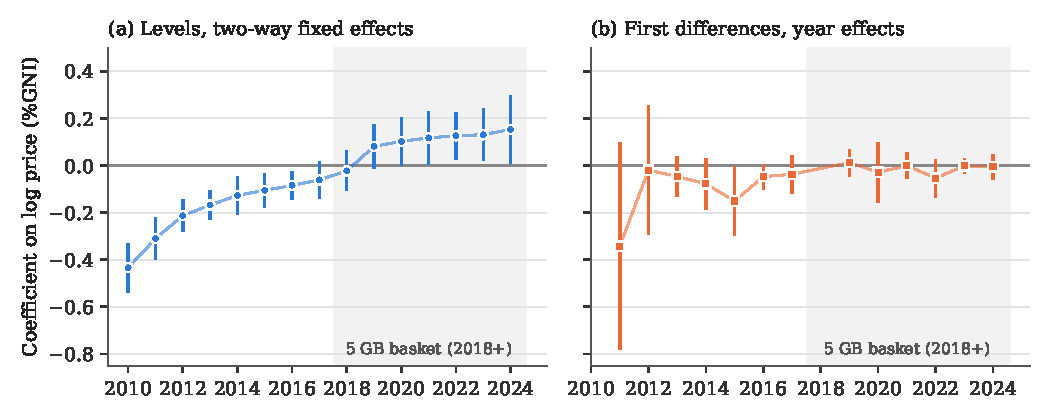
\includegraphics[width=\textwidth]{fig1_yearly_slopes.pdf}
\caption{Year-specific price coefficients, 33 countries. Panel~(a): log subscriptions per 100 inhabitants on log price interacted with year indicators, with country and year effects and core controls. Panel~(b): the same in first differences with year effects; the 2017--2018 change is excluded because the basket definition changed, and 2019 is estimated only for the 11 countries with a new 2019 price. Bars are 95\% confidence intervals with standard errors clustered by country. Shaded area: 5\,GB basket (from 2018)}\label{fig:yearly}
\end{figure}

\begin{table}[t]
\caption{Pooled price coefficient: levels versus within-differenced and dynamic estimators}\label{tab:pooled}
\footnotesize\setlength{\tabcolsep}{3pt}
\begin{tabular*}{\textwidth}{@{\extracolsep{\fill}}lcccccc@{}}
\toprule
& (1) & (2) & (3) & (4) & (5) & (6) \\
& \shortstack{TWFE\\levels} & \shortstack{+ country\\trends} & \shortstack{First\\differences} & \shortstack{FD, 2-year\\cumulative} & \shortstack{Dynamic\\LSDV} & \shortstack{Difference\\GMM} \\
\midrule
\multicolumn{7}{@{}l}{\textit{Panel A. 2010--2019}}\\
Log price & $-0.23^{***}$ & $-0.08$ & $-0.07^{*}$ & $-0.11^{***}$ & $0.00$ & $-0.00$\\
 & (0.07) & (0.05) & (0.04) & (0.04) & (0.01) & (0.11)\\
WCR bootstrap $p$ & $<$0.001 & 0.158 & 0.080 & -- & -- & --\\
Lagged dependent variable & -- & -- & -- & -- & $0.61^{***}$ & $0.65^{***}$\\
Long-run effect & -- & -- & -- & -- & $0.00$ & $-0.00$ (0.32)\\
Hansen $J$ / AR(2) $p$ & -- & -- & -- & -- & -- & 0.62 / 0.45\\
Observations & 307 & 307 & 240 & 195 & 274 & 240\\
\midrule
\multicolumn{7}{@{}l}{\textit{Panel B. 2010--2024}}\\
Log price & $-0.13^{**}$ & $-0.06$ & $-0.05^{*}$ & $-0.06$ & $0.02$ & $-0.03$\\
 & (0.06) & (0.04) & (0.03) & (0.04) & (0.01) & (0.09)\\
WCR bootstrap $p$ & 0.058 & 0.206 & 0.075 & -- & -- & --\\
Lagged dependent variable & -- & -- & -- & -- & $0.72^{***}$ & $0.61^{***}$\\
Long-run effect & -- & -- & -- & -- & $0.06$ & $-0.07$ (0.21)\\
Hansen $J$ / AR(2) $p$ & -- & -- & -- & -- & -- & 0.64 / 0.79\\
Observations & 471 & 471 & 382 & 315 & 438 & 382\\
\botrule
\end{tabular*}
\footnotetext{Dependent variable: log fixed-broadband subscriptions per 100 inhabitants (first-differenced in columns 3--4, 6). Price: log entry-level basket as \% of GNI per capita. Columns 1--2 include country and year effects; columns 3--4 include year effects; all include the core controls of Section~\ref{sec:data}. Column 2 adds country-specific linear trends. Column 4 reports the sum of the current and lagged price-change coefficients. Column 5 adds the lagged dependent variable to column 1 (the short-run coefficient is shown; Nickell bias is of order $1/T$). Column 6 is one-step difference GMM with price treated as endogenous, instruments collapsed and limited to lags 2--3 (12 instruments in Panel A, 17 in Panel B), log GDP per capita as the only control and year effects; long-run standard error by the delta method. Carried-forward 2019 prices are treated as missing and the 2017--2018 change is excluded in columns 3--4. Standard errors clustered by country (33 clusters) in parentheses. WCR: wild cluster restricted bootstrap $p$-value, Webb weights, 9{,}999 replications. $^{*}p<0.10$, $^{**}p<0.05$, $^{***}p<0.01$.}
\end{table}


\subsection{EU and Eastern Partnership countries}

Table~\ref{tab:groups} separates the two groups for 2010--2019. In the EU the price coefficient is $-0.08$ in levels and between $-0.04$ and $0.00$ in every other column. In first differences its 90\% confidence interval is $[-0.04, 0.02]$, and two one-sided tests reject the hypothesis that it lies outside $\pm 0.10$ ($p<0.001$). Long differences give $-0.04$ (three years) and $-0.06$ (five years), so measurement error in annual price changes does not appear to conceal a sizeable EU coefficient.

In the EaP the coefficient is $-0.46$ in levels, $-0.27$ with trends, $-0.28$ in first differences and $-0.17$ when country effects are added to the first-difference model. It is $-0.45$ in three-year and $-0.46$ in five-year differences. The EaP--EU difference is significant under cluster-robust inference in columns 1--4 and under randomisation inference in columns 1--3 ($p$-values 0.03, 0.03 and 0.005); the wild bootstrap gives 0.01, 0.09, 0.04 and 0.13. Leaving out one EaP country at a time keeps the first-difference coefficient between $-0.34$ and $-0.20$.

Column~5 shows what these estimates rest on. When the year effects are allowed to differ between the two groups, the EaP coefficient is identified only from the question whether, within a year, the EaP countries whose affordability improved more also saw faster adoption. The answer is no: the coefficient is $+0.13$ (standard error 0.13). The negative coefficients in columns 1--4 therefore come from movements common to the six EaP countries. In the years in which EaP affordability improved most, EaP adoption grew fastest: average EaP penetration grew by 36 and 29 log points in 2011 and 2012, while the affordability ratio fell by about 20 log points in each year, and both movements slowed thereafter (Online Resource, Table~S7, reports the EaP coefficient year by year). Because the common year effects are estimated mainly from EU countries, this bloc-wide co-movement enters the price coefficient. It amounts to one time series of about seven annual observations, shared by six countries, and it is equally consistent with a common catch-up in which incomes, networks and tariffs moved together.

Figure~\ref{fig:slopes} plots the country-specific first-difference slopes. Five of the six EaP slopes are negative, Georgia's is positive and imprecise, and the EU slopes are concentrated around zero, with Lithuania and Czechia the most negative. The unweighted mean of the EaP slopes is $-0.19$ with a standard error of 0.20; the precision-weighted mean is $-0.25$, but Belarus alone carries 48\% of its weight. The distribution of EaP slopes differs from that of EU slopes according to a two-sided rank-sum test ($p=0.02$) but not according to a permutation test of the means ($p=0.08$). In the levels regression the six EaP countries account for 32\% of the residual price variation from which the coefficient is estimated, far more than their share of the sample.

\begin{figure}[t]
\centering
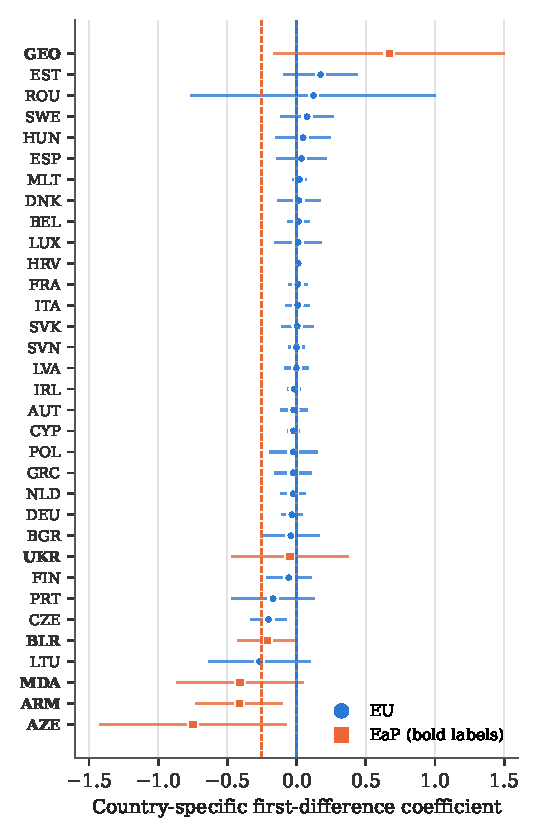
\includegraphics[width=0.62\textwidth]{fig2_country_slopes.pdf}
\caption{Country-specific first-difference slopes, 2010--2019. Each slope comes from a regression of the annual change in log subscriptions per 100 inhabitants on the change in log price and in log GDP per capita, with 7--8 observations per country (5 for Romania); bars are 95\% confidence intervals. Squares and bold labels: EaP countries. Dashed lines: inverse-variance-weighted group means (EU near zero; EaP $-0.25$)}\label{fig:slopes}
\end{figure}

\begin{table}[t]
\caption{Price coefficients for EU and Eastern Partnership countries, 2010--2019}\label{tab:groups}
\scriptsize\setlength{\tabcolsep}{1pt}
\begin{tabular*}{\textwidth}{@{\extracolsep{\fill}}lccccccc@{}}
\toprule
& (1) & (2) & (3) & (4) & (5) & (6) & (7) \\
& \shortstack{TWFE\\levels} & \shortstack{+ country\\trends} & \shortstack{First\\differences} & \shortstack{FD +\\country FE} & \shortstack{FD + group\\year FE} & \shortstack{3-year\\diff.} & \shortstack{Mean\\group} \\
\midrule
EU & $-0.08^{*}$ & $-0.01$ & $-0.01$ & $-0.00$ & $-0.00$ & $-0.04$ & $-0.01$\\
 & (0.05) & (0.03) & (0.02) & (0.02) & (0.01) & (0.03) & (0.02)\\
EaP & $-0.46^{***}$ & $-0.27^{***}$ & $-0.28^{***}$ & $-0.17^{**}$ & $0.13$ & $-0.45^{***}$ & $-0.19$\\
 & (0.09) & (0.09) & (0.08) & (0.08) & (0.13) & (0.10) & (0.20)\\
\midrule
\multicolumn{8}{@{}l}{\textit{$p$-values for the EaP--EU difference}}\\
Cluster-robust & $<$0.001 & 0.004 & $<$0.001 & 0.035 & 0.291 & & \\
Wild bootstrap & 0.012 & 0.095 & 0.037 & 0.133 & 0.523 & & \\
Randomisation & 0.026 & 0.028 & 0.005 & & & & 0.084\\
Rank-sum & & & & & & & 0.021\\
Observations & 307 & 307 & 240 & 240 & 240 & 163 & 33\\
\botrule
\end{tabular*}
\footnotetext{Columns 1--6 are single regressions in which the price coefficient is interacted with an EaP indicator; the EaP row reports the sum of the main and interaction coefficients. Column 4 adds country effects to the first-difference model (country-specific trends in levels). Column 5 replaces the common year effects by year effects specific to each group, so that the EaP coefficient is identified only from differences among the six EaP countries within a year. Column 6 uses overlapping 3-year differences within the 2010--2017 basket regime, with year effects (5-year differences: EU $-0.06$, EaP $-0.46$). Column 7 is the unweighted average of country-specific first-difference slopes \citep{pesaran1995estimating} with the standard error from their dispersion; the inverse-variance-weighted averages are $-0.00$ (EU) and $-0.25$ (EaP), the latter with 48\% of the weight on Belarus; its $p$-values come from permuting group labels across the 33 slopes and from a two-sided Mann--Whitney test. Randomisation inference reassigns the EaP label to 6 of the 33 countries at random (4{,}999 draws) and compares studentised statistics. Wild bootstrap: WCR, Webb weights. Range of the EaP coefficient when one EaP country is left out: (1) $-0.54$ to $-0.40$; (2) $-0.35$ to $-0.21$; (3) $-0.34$ to $-0.20$. Other notes as in Table~\ref{tab:pooled}.}
\end{table}


\subsection{Timing: basket definitions, sub-periods and the period after 2019}

Table~\ref{tab:timing} asks whether the coefficient changed over time. Panel~A estimates the pooled model separately under the two basket definitions. Under the 1\,GB basket (2010--2017) the levels coefficient is $-0.24$ and the first-difference coefficient $-0.09$; under the 5\,GB basket (2018--2024) both are zero, the first-difference coefficient precisely so ($-0.004$, standard error 0.009). Because the revision coincides with the years in which the levels coefficient in Figure~\ref{fig:yearly} changes sign, a comparison of levels estimates across 2018 mixes a change in the price concept with any change in behaviour.

Panel~B splits the first-difference sample. The EaP coefficient is $-0.29$ in 2011--2013, $-0.04$ in 2014--2017 and $-0.02$ in 2019--2024, and none of these differs significantly from the EU coefficient. Sub-period estimates of this kind are sensitive to the choice of years, because the controls are re-estimated within each window and each window contains only a few years of the common EaP movement described above: for 2011--2016 the EaP coefficient is $-0.32$, for 2014--2016 $-0.04$. The EU coefficient is indistinguishable from zero in every sub-period.

Panel~C addresses the question that motivated earlier work on this panel, whether the price coefficient changed after 2019. In levels the interaction of price with the 2020--2024 indicator is $+0.30$ and highly significant, and the model with separate groups attributes most of this shift to the EaP ($+0.38$). With country trends the pooled shift is $-0.08$ (WCR $p=0.23$); in the version with separate groups the EU shift is also $-0.08$ and is significant (WCR $p=0.008$), which, if anything, points to a slightly more negative EU coefficient after 2019. In first differences the pooled shift is $+0.05$ (WCR $p=0.04$), moving the coefficient from $-0.07$ to $-0.01$; by group, the shifts are $+0.01$ for the EU (WCR $p=0.72$) and $+0.09$ for the EaP (WCR $p=0.05$). Excluding Ukraine from 2022 and Belarus from 2020, or ending the sample in 2021 so as to leave out the war in Ukraine and the rapid spread of generative-AI applications, does not change these results (Online Resource, Table~S3). Including 2020--2024 thus moves the levels coefficient towards zero because it adds years late in the catch-up; in the specifications that are robust to diffusion there is no sign of the weakening of the price response after 2020 that the levels regression suggests.

\begin{table}[t]
\caption{Did the price response change? Basket regimes, sub-periods and the post-2019 period}\label{tab:timing}
\footnotesize\setlength{\tabcolsep}{3pt}
\begin{tabular*}{\textwidth}{@{\extracolsep{\fill}}lccccc@{}}
\toprule
\multicolumn{6}{@{}l}{\textit{Panel A. Pooled coefficient within each ITU basket regime}}\\
& \multicolumn{2}{c}{1\,GB basket, 2010--2017} & \multicolumn{2}{c}{5\,GB basket, 2018--2024} & \\
\cmidrule(lr){2-3}\cmidrule(lr){4-5}
& TWFE levels & First differences & TWFE levels & First differences & \\
Log price & $-0.24^{***}$ & $-0.09^{*}$ & $0.00$ & $-0.00$ & \\
& (0.08) & (0.05) & (0.03) & (0.01) & \\
Observations & 263 & 229 & 208 & 153 & \\
\midrule
\multicolumn{6}{@{}l}{\textit{Panel B. First differences by sub-period}}\\
& 2011--2013 & 2014--2017 & 2019--2024 & & \\
EU & $0.05$ & $-0.01$ & $-0.00$ & & \\
& (0.05) & (0.01) & (0.01) & & \\
EaP & $-0.29$ & $-0.04$ & $-0.02$ & & \\
& (0.18) & (0.04) & (0.05) & & \\
EaP--EU: WCR / RI $p$ & 0.38 / 0.16 & 0.61 / 0.62 & 0.81 / 0.81 & & \\
Observations & 98 & 131 & 153 & & \\
\midrule
\multicolumn{6}{@{}l}{\textit{Panel C. Price $\times$ post-2019 (2020--2024), full sample}}\\
& \multicolumn{2}{c}{TWFE levels} & + country trends & First differences & \\
Log price & \multicolumn{2}{c}{$-0.22^{***}$} & $-0.03$ & $-0.07^{**}$ & \\
& \multicolumn{2}{c}{(0.05)} & (0.05) & (0.03) & \\
Log price $\times$ post-2019 & \multicolumn{2}{c}{$0.30^{***}$} & $-0.08$ & $0.05^{**}$ & \\
& \multicolumn{2}{c}{(0.07)} & (0.06) & (0.02) & \\
WCR $p$, shift & \multicolumn{2}{c}{$<$0.001} & 0.226 & 0.043 & \\
Post-2019 coefficient & \multicolumn{2}{c}{$0.08$} & $-0.11^{***}$ & $-0.01$ & \\
Shift, EU / EaP & \multicolumn{2}{c}{0.11 / 0.38} & $-$0.08 / $-$0.10 & 0.01 / 0.09 & \\
WCR $p$, EU / EaP shift & \multicolumn{2}{c}{0.087 / 0.003} & 0.008 / 0.682 & 0.717 / 0.053 & \\
Observations & \multicolumn{2}{c}{471} & 471 & 382 & \\
\botrule
\end{tabular*}
\footnotetext{Panel A estimates the pooled model separately within the two ITU basket definitions. Panel B interacts the price change with an EaP indicator within each sub-period; WCR and RI $p$-values refer to the EaP--EU difference. Panel C interacts price with an indicator for 2020--2024; the split model interacts it further with the EaP indicator. Other notes as in Table~\ref{tab:pooled}.}
\end{table}


\subsection{What lies behind the EaP coefficient?}

Table~\ref{tab:eapchecks} examines the first-difference EaP coefficient further. It depends on the price concept: with PPP prices it is $-0.10$ and imprecise, with US-dollar prices $-0.23$ ($p=0.06$), and with the affordability ratio $-0.28$. Row~5 replaces the ratio by its two components, the US-dollar tariff and the Atlas GNI per capita implied by ITU's ratio. With log GDP per capita as a control, the EaP tariff coefficient is $-0.26$ ($p=0.02$) and the GNI coefficient $+0.36$ ($p=0.01$); the restriction that they are equal and opposite, which a pure affordability effect implies, is not rejected ($p=0.66$). Without the GDP control the tariff coefficient falls to $-0.15$ and loses significance, while the GNI coefficient rises to $+0.51$. For the EU the tariff coefficient is zero, the GNI coefficient is $-0.34$ and the restriction is rejected ($p=0.03$). Atlas GNI in US dollars moves with exchange rates, so in both groups the income denominator partly measures currency movements rather than income, and the coefficient on the ratio should not be read as a pure tariff effect. Dropping the EaP country-years of the 2014--2016 currency crises lowers the EaP coefficient to $-0.22$ ($p=0.05$).

Other checks leave the EaP coefficient between $-0.22$ and $-0.30$: excluding Azerbaijan, whose slope is the largest; replacing GDP by night-time lights ($-0.22$, $p=0.03$); restricting the controls to GDP; adding servers and research spending; using Internet users as the outcome ($-0.27$); and using the logistic transformation of penetration ($-0.30$). None of these checks removes the common EaP movement on which the coefficient rests. The timing placebo in row~16 shows that next year's price change also has a negative coefficient for the EaP ($-0.16$, $p=0.11$), while the current change keeps its coefficient of $-0.27$. Adoption growth and future affordability gains are thus related, as one would expect if both respond to common, slowly moving conditions.

\begin{table}[t]
\caption{First-difference estimates, 2010--2019: what drives the EaP coefficient?}\label{tab:eapchecks}
\footnotesize\setlength{\tabcolsep}{3pt}
\begin{tabular*}{\textwidth}{@{\extracolsep{\fill}}lccccc@{}}
\toprule
& \multicolumn{2}{c}{EaP} & \multicolumn{2}{c}{EU} & \\
\cmidrule(lr){2-3}\cmidrule(lr){4-5}
Specification & Coef. & SE & Coef. & SE & Obs. \\
\midrule
(1) Baseline & $-0.28^{***}$ & (0.08) & $-0.01$ & (0.02) & 240\\
\multicolumn{6}{@{}l}{\textit{Price measurement}}\\
(2) Price in PPP dollars & $-0.10$ & (0.23) & $-0.02$ & (0.02) & 233\\
(3) Price in current US dollars & $-0.23^{*}$ & (0.12) & $-0.02$ & (0.02) & 242\\
(4) Incl.\ repeated 2019 prices, 2017--18 change & $-0.27^{***}$ & (0.08) & $-0.01$ & (0.01) & 295\\
\multicolumn{6}{@{}l}{\textit{Decomposing the affordability ratio (with log GDP per capita)}}\\
(5a) Log tariff, US\$ & $-0.26^{**}$ & (0.11) & $-0.02$ & (0.02) & \\
(5b) Log GNI p.c.\ (ITU denominator) & $0.36^{**}$ & (0.15) & $-0.34^{**}$ & (0.15) & \\
(5c) Test tariff $+$ GNI $=0$, $p$ & \multicolumn{2}{c}{0.66} & \multicolumn{2}{c}{0.03} & \\
(6a) Log tariff, US\$, no GDP control & $-0.15$ & (0.14) & $-0.01$ & (0.01) & \\
(6b) Log GNI p.c., no GDP control & $0.51^{***}$ & (0.16) & $-0.04$ & (0.11) & \\
\multicolumn{6}{@{}l}{\textit{Sample and controls}}\\
(7) Excl.\ currency-crisis years & $-0.22^{*}$ & (0.12) & $-0.02$ & (0.02) & 231\\
(8) Excluding Azerbaijan & $-0.27^{***}$ & (0.10) & $-0.00$ & (0.02) & 233\\
(9) Night lights instead of GDP & $-0.22^{**}$ & (0.10) & $0.01$ & (0.02) & 208\\
(10) Night lights and GDP & $-0.27^{***}$ & (0.07) & $-0.00$ & (0.02) & 208\\
(11) Log GDP per capita only & $-0.27^{***}$ & (0.07) & $-0.01$ & (0.02) & 240\\
(12) Adding secure servers and R\&D & $-0.25^{***}$ & (0.09) & $0.00$ & (0.02) & 240\\
\multicolumn{6}{@{}l}{\textit{Outcome and functional form}}\\
(13) Internet users (\%) & $-0.27^{***}$ & (0.03) & $-0.03^{*}$ & (0.01) & 240\\
(14) Log count of subscriptions & $-0.26^{***}$ & (0.08) & $-0.01$ & (0.01) & 295\\
(15) Log-odds, ceiling 70 per 100 & $-0.30^{***}$ & (0.08) & $-0.01$ & (0.02) & 240\\
\multicolumn{6}{@{}l}{\textit{Timing}}\\
(16a) Current price change & $-0.27^{***}$ & (0.08) & $-0.01$ & (0.03) & 195\\
(16b) Next year's price change & $-0.16$ & (0.10) & $-0.01$ & (0.02) & \\
\botrule
\end{tabular*}
\footnotetext{All rows are first-difference regressions with year effects and core controls unless stated, 2010--2019, clustered standard errors (33 countries). Row 5 replaces the log affordability ratio by its two components, the US-dollar tariff and the Atlas GNI per capita implied by ITU's ratio; under a pure affordability response their coefficients are equal and opposite. Row 7 drops Azerbaijan 2015--16, Ukraine 2014--15, Belarus 2011 and 2015, and Armenia, Georgia and Moldova 2015. Night lights: harmonised DMSP/VIIRS radiance summed over national territory (\citealp{li2020harmonized}, 2024 release); the 2013--2014 sensor change is excluded. Row 15: $\ln[s/(70-s)]$. Row 16 adds next year's price change; the EaP coefficient on the current change in 16a is the sum of main and interaction terms. $^{*}p<0.10$, $^{**}p<0.05$, $^{***}p<0.01$.}
\end{table}


\subsection{Regional evidence}

The EU result could conceal price sensitivity in poorer regions if richer regions in the same country do not respond. Table~\ref{tab:regional} uses the regional panel to test this. The national price has no detectable association with the regional share of households with broadband ($0.03$, standard error 0.04). Its interaction with the indicator of a less-developed region is $-0.02$ with region and year effects, and $0.03$ with country-by-year effects, which absorb all national shocks including the national price itself. For 2010--2017 the interaction is $-0.06$. None of these estimates is significant, but the 95\% confidence interval for the interaction, $[-0.18, 0.14]$, includes differences of moderate size. The regional data thus give no support to the view that the EU result masks a large response in less-developed regions, but they cannot rule out a moderate one, and they cannot address low-income households within regions.

\begin{table}[t]
\caption{Regional evidence: households with broadband in 175 EU regions, 2010--2021}\label{tab:regional}
\footnotesize\setlength{\tabcolsep}{3pt}
\begin{tabular*}{\textwidth}{@{\extracolsep{\fill}}lccccc@{}}
\toprule
& (1) & (2) & (3) & (4) & (5) \\
FE & \shortstack{Region,\\year} & \shortstack{Region,\\year} & \shortstack{Region,\\country-year} & \shortstack{Region,\\country-year} & \shortstack{Region, year\\2010--2017} \\
\midrule
National log price & $0.03$ & $0.03$ & -- & -- & $0.02$\\
& (0.04) & (0.05) & & & (0.07)\\
Price $\times$ less-developed & & $-0.02$ & $0.03$ & $0.01$ & $-0.06$\\
& & (0.08) & (0.07) & (0.08) & (0.12)\\
Price $\times$ less-dev. $\times$ 2020--21 & & & & $0.08^{*}$ & \\
& & & & (0.05) & \\
WCR $p$ (first coef.) & 0.573 & 0.765 & 0.786 & 0.936 & 0.616\\
Observations & 1807 & 1807 & 1807 & 1807 & 1218\\
\botrule
\end{tabular*}
\footnotetext{Dependent variable: log share of households with broadband (Eurostat \texttt{isoc\_r\_broad\_h}), finest regional level available (NUTS-2; NUTS-1 for Germany, Greece and Poland), 19 member states with at least two regions. National price: log ITU basket as \% of GNI per capita. Less-developed region: GDP per head in PPS below 75\% of the EU average in the first observed year (46 regions), the EU cohesion-policy threshold. All columns control for log regional GDP per head in PPS; columns 1, 2 and 5 also for national log GDP per capita. Standard errors clustered by member state (19 clusters); WCR with 1{,}999 replications. The 95\% confidence interval for the interaction in column 2 is $[-0.18, 0.14]$. $^{*}p<0.10$, $^{**}p<0.05$, $^{***}p<0.01$.}
\end{table}


\subsection{Further checks}\label{sec:further}

The Online Resource reports further checks. The results are unchanged when the repeated 2019 prices and the 2017--2018 change are included, when the outcome is the log count of subscriptions, with Driscoll--Kraay standard errors, and when secure servers and research and development expenditure are added to the controls. In first differences the EaP elasticity at the group means is $-0.21$ in the log-linear form, $-0.04$ in the linear form and $-0.12$ in the linear-log form; only the first is significant, while the EU value is zero in all three. When the price coefficient is allowed to vary with headroom, the pooled interaction is $-0.69$ ($p=0.05$), so the coefficient is larger in absolute value where penetration is further from the ceiling; once the EaP interaction is added, the headroom interaction falls to $-0.19$ and is insignificant, because low penetration and EaP membership nearly coincide in this sample. The mobile-broadband basket is available only from 2013, so controlling for it restricts the sample to 2014--2019, years in which no EaP coefficient is found with or without the control.

\section{Discussion}\label{sec:discussion}

\subsection{What the country panel identifies}

A panel in which late adopters start with high prices and then catch up attributes part of the catch-up to price in levels, and its year-specific version produces a steady attenuation of the price coefficient, which the ITU basket revision turns into a change of sign. Trend-robust and differenced estimators remove most of this pattern. The same mechanism is likely to affect cross-country studies of any good in the middle of its diffusion. Levels regressions of this kind should therefore be reported together with trend-robust, differenced and country-specific estimates, and year-specific levels coefficients should not be used to date changes in price sensitivity. Revisions of price concepts, such as the 2018 basket change and the repeated 2019 values, need to be handled explicitly.

After these corrections the panel shows two things. In the EU, aggregate adoption was not associated with entry-level prices in 2010--2024. This agrees with the small adoption effects of large US subsidies \citep{mendez2021lifeline} and with the view that, where most households are connected and basic access is cheap relative to income, those still unconnected are held back by other factors. In the EaP, adoption and affordability improved together, most strongly in the early 2010s, when penetration was low and entry-level broadband cost more than 4\% of GNI per capita, twice the Broadband Commission threshold. The panel cannot say whether affordability caused the adoption. The co-movement is common to the six countries; it does not appear within the group, it partly reflects the income denominator, and future price changes are also associated with current adoption growth.

\subsection{Saturation or necessity?}

A zero coefficient may mean that demand has become insensitive to price because broadband is now a necessity, or that few households remain at the margin because the market is close to saturation. Aggregate data cannot fully separate the two. Three observations favour saturation as the main reason in the EU. The coefficient is larger in absolute value where headroom is larger, although in this sample headroom is hard to separate from EaP membership (Section~\ref{sec:further}). In the EU, where penetration was already high in 2010, no association is found in any sub-period, including the early 2010s. And the logistic specification, which builds a ceiling into the functional form, gives the same conclusions. A test of necessity would require countries with low penetration after 2014, and the sample contains too few.

\subsection{Comparison with other essential services}

For comparison, the meta-analysis of \citet{labandeira2017meta} reports a mean short-run price elasticity of energy demand of about $-0.2$ and a long-run elasticity of about $-0.65$, and that of \citet{dalhuisen2003price} a mean price elasticity of residential water demand of about $-0.4$ \citep[see also][]{espey2004turn}. These elasticities describe the quantity consumed by connected households, whereas ours concern the decision to connect, so the comparison is only indicative. The EU coefficient is smaller than typical estimates for energy or water. The EaP coefficients are of the same order, but they are not causal estimates.

\subsection{Regulatory implications}

Three implications follow, each limited by the aggregate nature of the evidence. First, in EU markets the data give no reason to expect that lower entry-level prices would raise aggregate adoption much. This does not make the affordability provisions of the European Electronic Communications Code redundant: targeted measures are aimed at households for whom price does bind, and a national average cannot reveal their behaviour. It does suggest that efforts to raise adoption further should also address availability, quality and skills, and that their evaluation needs household or regional microdata. The end of the US Affordable Connectivity Program in 2024 offers such an opportunity \citep{fcc_acp}. Second, for markets where penetration is low and basic access costs several percent of income, the EaP experience of the early 2010s shows that adoption and affordability can improve rapidly together, but a country panel cannot tell how much of the adoption was due to prices. Regulators in such markets need evidence at the household level before relying on price measures. Third, the price coefficient had already vanished in the robust specifications before 2020, and the panel gives no evidence that the pandemic changed it. We conjecture that the pandemic changed the attention that policy makers paid to broadband more than it changed household behaviour.

\subsection{Limitations}

The analysis has four main limitations. Aggregate data cannot reveal the price sensitivity of particular households, and the regional evidence narrows this gap only partly. The entry-level basket is a single plan of one operator and becomes less representative as subscribers move to faster plans, so a response to the prices that subscribers actually pay could exist where none is found for entry-level prices. We have no credible instrument for price. Finally, the years after 2021 include the war in Ukraine and sanctions affecting Belarus, which are likely to have reduced the reliability of data for these countries; our results for 2020--2024 do not depend on the affected country-years.

\section{Conclusion}\label{sec:conclusion}

Country panels are the most widely available evidence on how broadband adoption responds to price. For the EU and its eastern neighbours in 2010--2024, the standard levels regression suggests a sizeable price response that fades over time. The fading is what heterogeneous diffusion produces even without any price effect, and the basket revision of 2018 adds a change of sign. Estimators that are robust to diffusion find no association between entry-level prices and adoption in the EU. In the Eastern Partnership they find an association that is common to the six countries, concentrated in the early 2010s, and absent within the group. Neither result identifies a causal price response. Cross-country regressions should therefore not be used to date changes in price sensitivity, and affordability policy should rest on household and regional evidence.

\backmatter

\bmhead{Supplementary information}
Online Resource~1 contains additional tables and a figure: alternative price concepts, controls and outcomes; Driscoll--Kraay standard errors; functional form and headroom; samples for the post-2019 test; Hausman-type instrumental-variable estimates; country-specific slopes and TWFE weights; the EaP coefficient by year; the construction of the data; and the simulation described in Section~\ref{sec:method}.

\ifblind\else
\bmhead{Acknowledgements}
The authors thank Daniel Vertesy and Esperanza Magpantay of the ITU Statistics Division for clarifications on the price baskets, and the referees of an earlier version for comments that shaped this article. The views expressed are those of the authors and do not necessarily reflect those of the Information Communication Technologies Agency of the Republic of Azerbaijan.
\fi

\section*{Declarations}

\begin{itemize}
\item \textbf{Funding:} No funding was received for conducting this study.
\item \textbf{Competing interests:} The authors have no competing interests to declare.
\item \textbf{Data availability:} All data are public: ITU ICT Price Baskets 2008--2025; World Bank WDI and WGI (July 2026 release); Eurostat \texttt{isoc\_r\_broad\_h} and \texttt{nama\_10r\_2gdp}; the harmonised night-time light series of \citet{li2020harmonized}. The analysis panel, the code and a record of every data transformation are available \ifblind from the authors on request\else at \url{https://github.com/sorujov/Broadband-Demand-Elasticity}\fi.
\item \textbf{Use of generative AI:} Generative AI tools were used to assist with coding, data checks and language editing. The authors reviewed all output and take full responsibility for the content.
\ifblind\else
\item \textbf{Author contributions:} S.O.: conceptualisation, methodology, software, formal analysis, data curation, writing (original draft and revision). I.I.: validation, writing (review and editing), supervision. J.H.: validation, writing (review and editing).
\fi
\end{itemize}

\bibliography{references}

\end{document}
